\section{Results}
\label{sec:results}

Every number in this section comes from one run per model per stage on one unit. They support statements about what happened in those runs; they do not rank the models in general.

\subsection{Before the Benchmark: Model-Only and Smoke Tests}

The model-only tests and the harness smoke test eliminated or flagged several candidates before stage~1, and they did not predict everything. \Mistral{} loaded and ran at 3 tokens per second, and with the weights resident it used 88~GiB at a 32,000-token context, so no context of 64,000 tokens or more fits beside it; it was not run in the harness. \Muse{} returned invalid JSON on the schema task and ran at 13 tokens per second. \Gptoss{} returned the wrong value from the long prompt three times, and in one of two smoke runs wrote a tool call as plain text and stopped after one turn. \Gthirtyone{} passed every format rule in the model-only tests, twice, and \Qeight{} followed every rule as well. \Gtwentysix{} twice broke two rules (a blank line before a list, and a p5.js call that fails when run), and \Nemo{} broke four. These results shaped expectations and did not decide the outcome: as Section~\ref{sec:discussion} shows, a model that follows every rule in isolation can still fail in the harness.

\subsection{Stage 1: Learning Graph}

Six of the ten models produced a learning graph. Table~\ref{tab:stage1} gives the structural result. All six graphs were acyclic and every JSON file matched its CSV. None of these checks says that the concepts are the right ones for Algebra~I or that the dependencies make sense; that judgment has not been made.

\begin{table}[htbp]
\centering
\footnotesize
{\setlength{\tabcolsep}{4pt}\begin{tabular}{@{}p{3.0cm}rrrrrp{4.7cm}@{}}
\toprule
\textbf{Model} & \textbf{Min.} & \textbf{Concepts} & \textbf{Deps} & \textbf{Calls (failed)} & \textbf{Peak (K)} & \textbf{Notable defects} \\
\midrule
\Qeight & 102 & 200 & 299 & 55 (1) & 108 & none structural \\
\Gthirtyone & 21 & 200 & 348 & 50 (8) & 68 & taxonomy page missing; navigation not updated \\
\Qsix & 22 & 200 & 273 & 55 (4) & 135 & 19 concepts with no prerequisite; 1 duplicate label \\
\Nemo & 18 & 199 & 494 & 140 (7) & 147 & one concept short; navigation not updated \\
\Gtwentysix & 6 & 200 & 483 & 51 (5) & 60 & 40 duplicate labels; index page missing; navigation not updated \\
\Gptoss & 17 & 200 & 180 & 28 (0) & 50 & 19 concepts connected to nothing \\
\midrule
\Granite & 150$^{\dagger}$ & --- & --- & 32 (4) & 50 & reached only the concept list \\
\Muse & 6 & --- & --- & 6 (0) & 125 & lost the task after a few steps \\
\Devstral & $<$1 & --- & --- & 0 & 21 & first tool call written as text \\
\Mistral & --- & --- & --- & --- & --- & not run: no usable context fits \\
\bottomrule
\end{tabular}}
\caption{Stage~1 results. Min.\ is wall-clock minutes; $^{\dagger}$ stopped at the 150-minute limit. ``Peak'' is the largest conversation, in thousands of tokens, that the server logged for that model. Calls are tool calls, with the number that failed in parentheses.}
\label{tab:stage1}
\end{table}

Two observations stand out. First, speed spans a factor of about 18: from 6 to 102 minutes for the same task, and from 6.7 to 111 seconds of wall-clock per tool call. The slowest model, \Qeight, produced the cleanest graph: exactly 200 concepts and 299 dependencies, two concepts with no prerequisite, no duplicate or overlong label, and a site that builds. Second, the models that produced a graph made between 28 and 140 tool calls. \Nemo{} needed 140, nearly three times as many as any other, and its conversation grew to 147,000 tokens.

\subsection{Stages 2 and 3: Chapter Structure and Chapter Text}

All six models that produced a graph completed stage~2 and designed between 10 and 14 chapters. Stage~3 is where they diverged (Figure~\ref{fig:completion}, Table~\ref{tab:stage3}). Two models, \Nemo{} and \Qsix, wrote every chapter they had designed. The other four stopped short, and \Qeight{} was too slow to write one.

\begin{figure}[htbp]
\centering
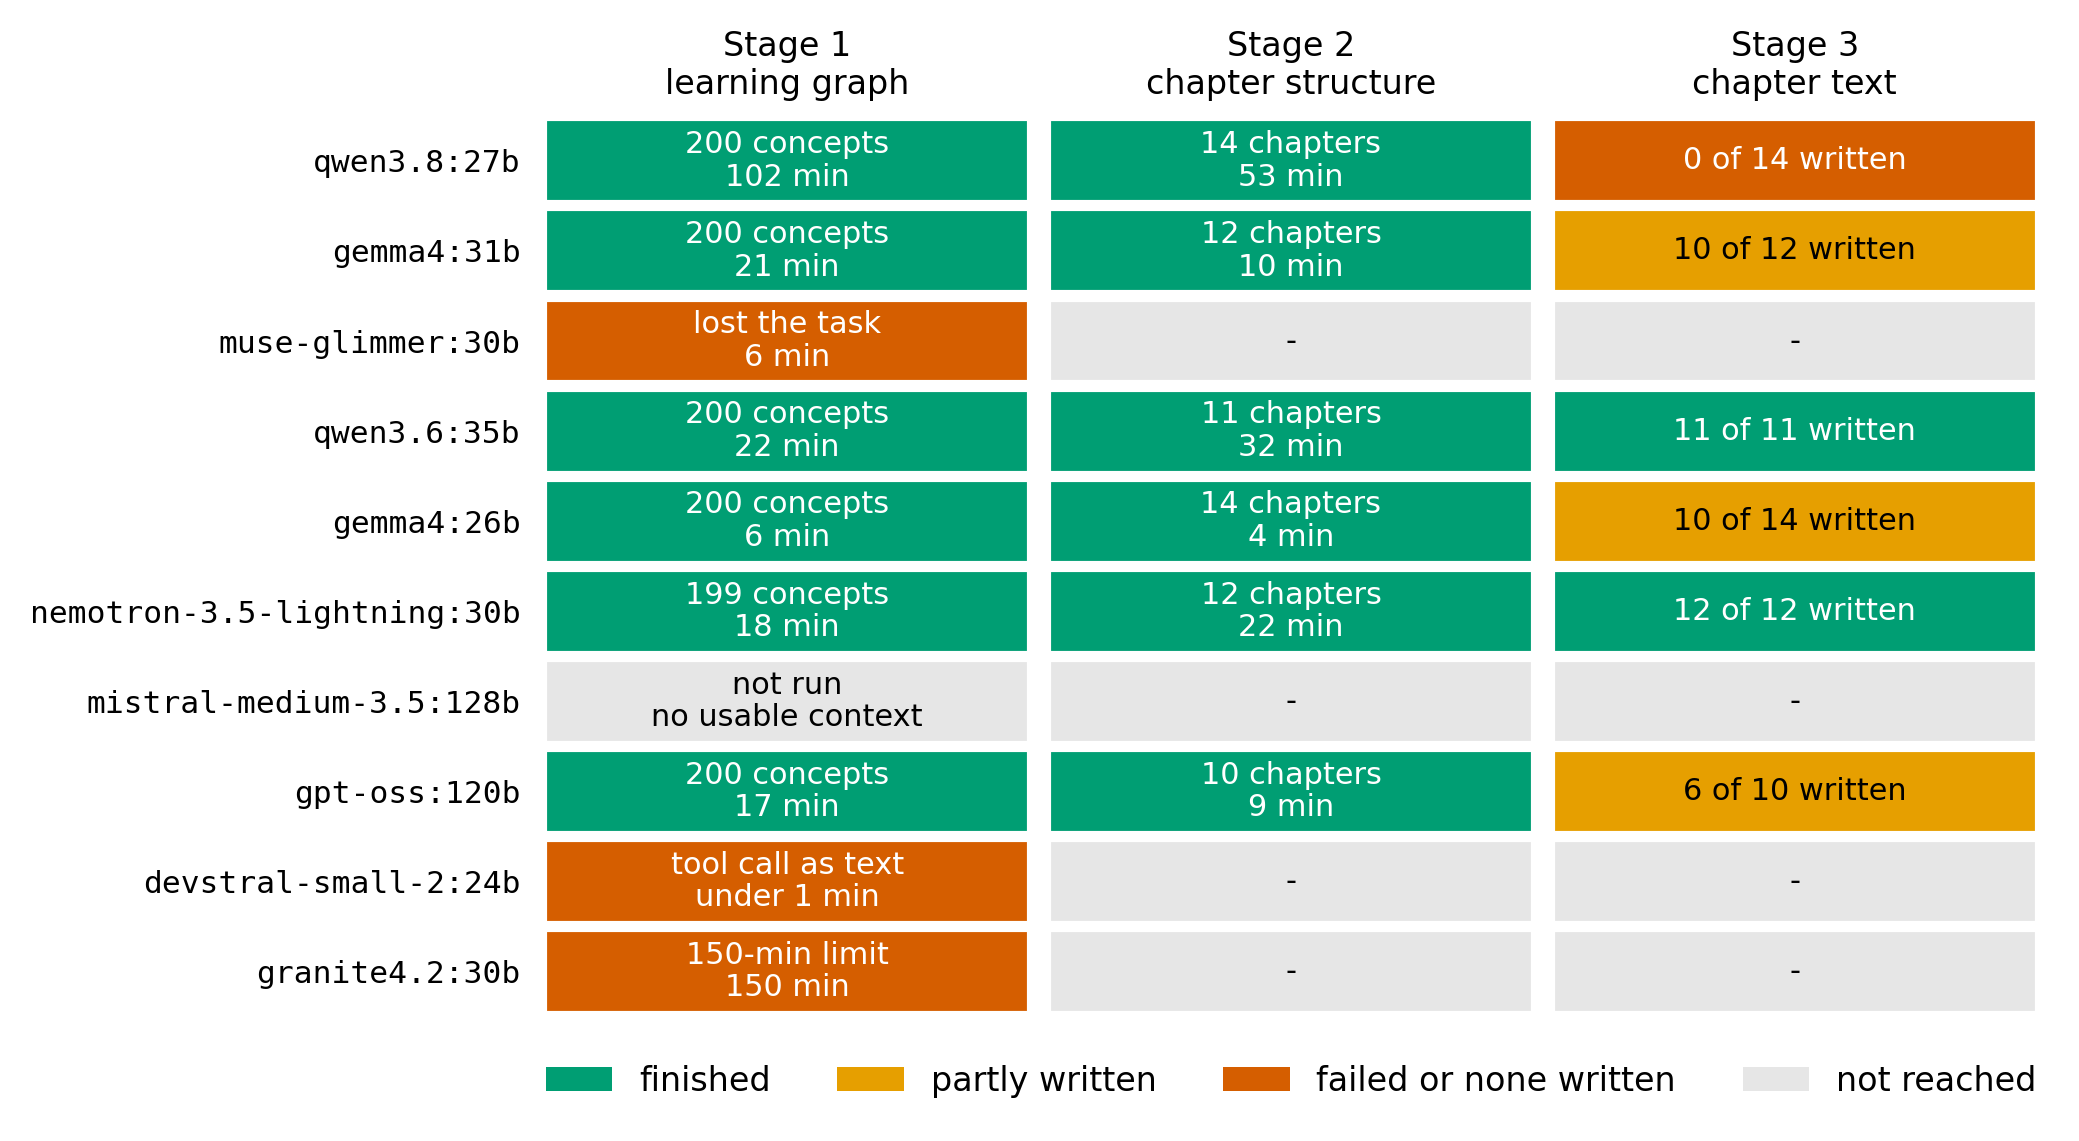
\includegraphics[width=0.95\textwidth]{figures/fig-completion.png}
\caption{How far each of the ten candidates got. Models are in the order in which they were chosen for testing, before any results. Cell text gives concept or chapter counts and wall-clock minutes for the one run.}
\label{fig:completion}
\end{figure}

\begin{table}[htbp]
\centering
\small
\begin{tabularx}{\textwidth}{@{}lrrrrX@{}}
\toprule
\textbf{Model} & \textbf{Designed} & \textbf{Stage 2} & \textbf{Written} & \textbf{Stage 3} & \textbf{Chapters not written} \\
\midrule
\Nemo & 12 & 22 min & 12 & 2.0 h & --- \\
\Qsix & 11 & 32 min & 11 & 1.3 h & --- \\
\Gthirtyone & 12 & 10 min & 10 & 4.3 h & 1 stopped at the 90-min limit; 1 ended on a stray control token \\
\Gtwentysix & 14 & 4 min & 10 & 1.7 h & 3 halted by the skill's own prerequisite check; 1 ended without writing \\
\Gptoss & 10 & 9 min & 6 & 1.5 h & 4 announced the skill, then ended the turn \\
\Qeight & 14 & 53 min & 0 & 3.0 h & 2 stopped at the limit; 12 not run \\
\bottomrule
\end{tabularx}
\caption{Stages~2 and~3. ``Designed'' is the number of chapters the model's own stage~2 output defined. Stage~3 time is the sum of the chapter runs.}
\label{tab:stage3}
\end{table}

\subsubsection{Failure Taxonomy}

The unfinished runs fail in a small number of recognizable ways (Table~\ref{tab:failures}). Most are failures of protocol or persistence and not of prose: the model did not produce a well-formed tool call, announced work instead of doing it, ran out of time, or lost the task as its conversation grew.

\begin{table}[htbp]
\centering
\footnotesize
\begin{tabular}{@{}p{2.7cm}p{7.0cm}p{4.6cm}@{}}
\toprule
\textbf{Failure} & \textbf{What was observed} & \textbf{Where} \\
\midrule
Tool call written as text & The first call appears as plain text; the harness sees no call and the run ends after one turn & \Devstral{} (both harness tests); \Gptoss{} (one smoke run) \\
Announces, does not act & The model says the skill is running, as if something else will do the work, and ends its turn without writing the chapter & \Gptoss: 4 of 10 chapters \\
Stray control token & The model's whole reply is a control token, not a tool call; the run ends after four turns & \Gthirtyone: 1 chapter \\
Ends without output & The run ends having written nothing & \Gtwentysix: 1 chapter \\
Self-inflicted precondition halt & The skill's own check finds that the chapter depends on concepts placed in later chapters, and the model stops as the skill requires; the cause is the model's own stage~2 design & \Gtwentysix: 3 chapters \\
Time limit & About twenty tool calls in 90 minutes without reaching the step that writes the file; or 150 minutes with only the concept list written & \Qeight: 2 chapters; \Granite{} (stage~1); \Gthirtyone: 1 chapter \\
Lost the task & The first prompt is 35,000 tokens against 17,000 to 21,000 for other models; within eight turns the conversation is at 120,000 tokens, the edge of its window, and the model answers with a greeting & \Muse \\
No usable context & The weights leave too little memory for a context of useful length & \Mistral \\
\bottomrule
\end{tabular}
\caption{Failure classes observed, with where each occurred.}
\label{tab:failures}
\end{table}

\subsection{Time and Effort}

Table~\ref{tab:effort} and Figure~\ref{fig:time} give machine time for the three stages. The fastest complete-or-partial books took 1.8 to 2.7 hours. \Gthirtyone{} took 4.8 hours, of which 1.5 hours was one chapter run that reached the 90-minute limit; excluding it, 3.3 hours. \Qeight{} spent 5.6 hours, 3.0 of them on two chapter runs that wrote nothing.

\begin{figure}[htbp]
\centering
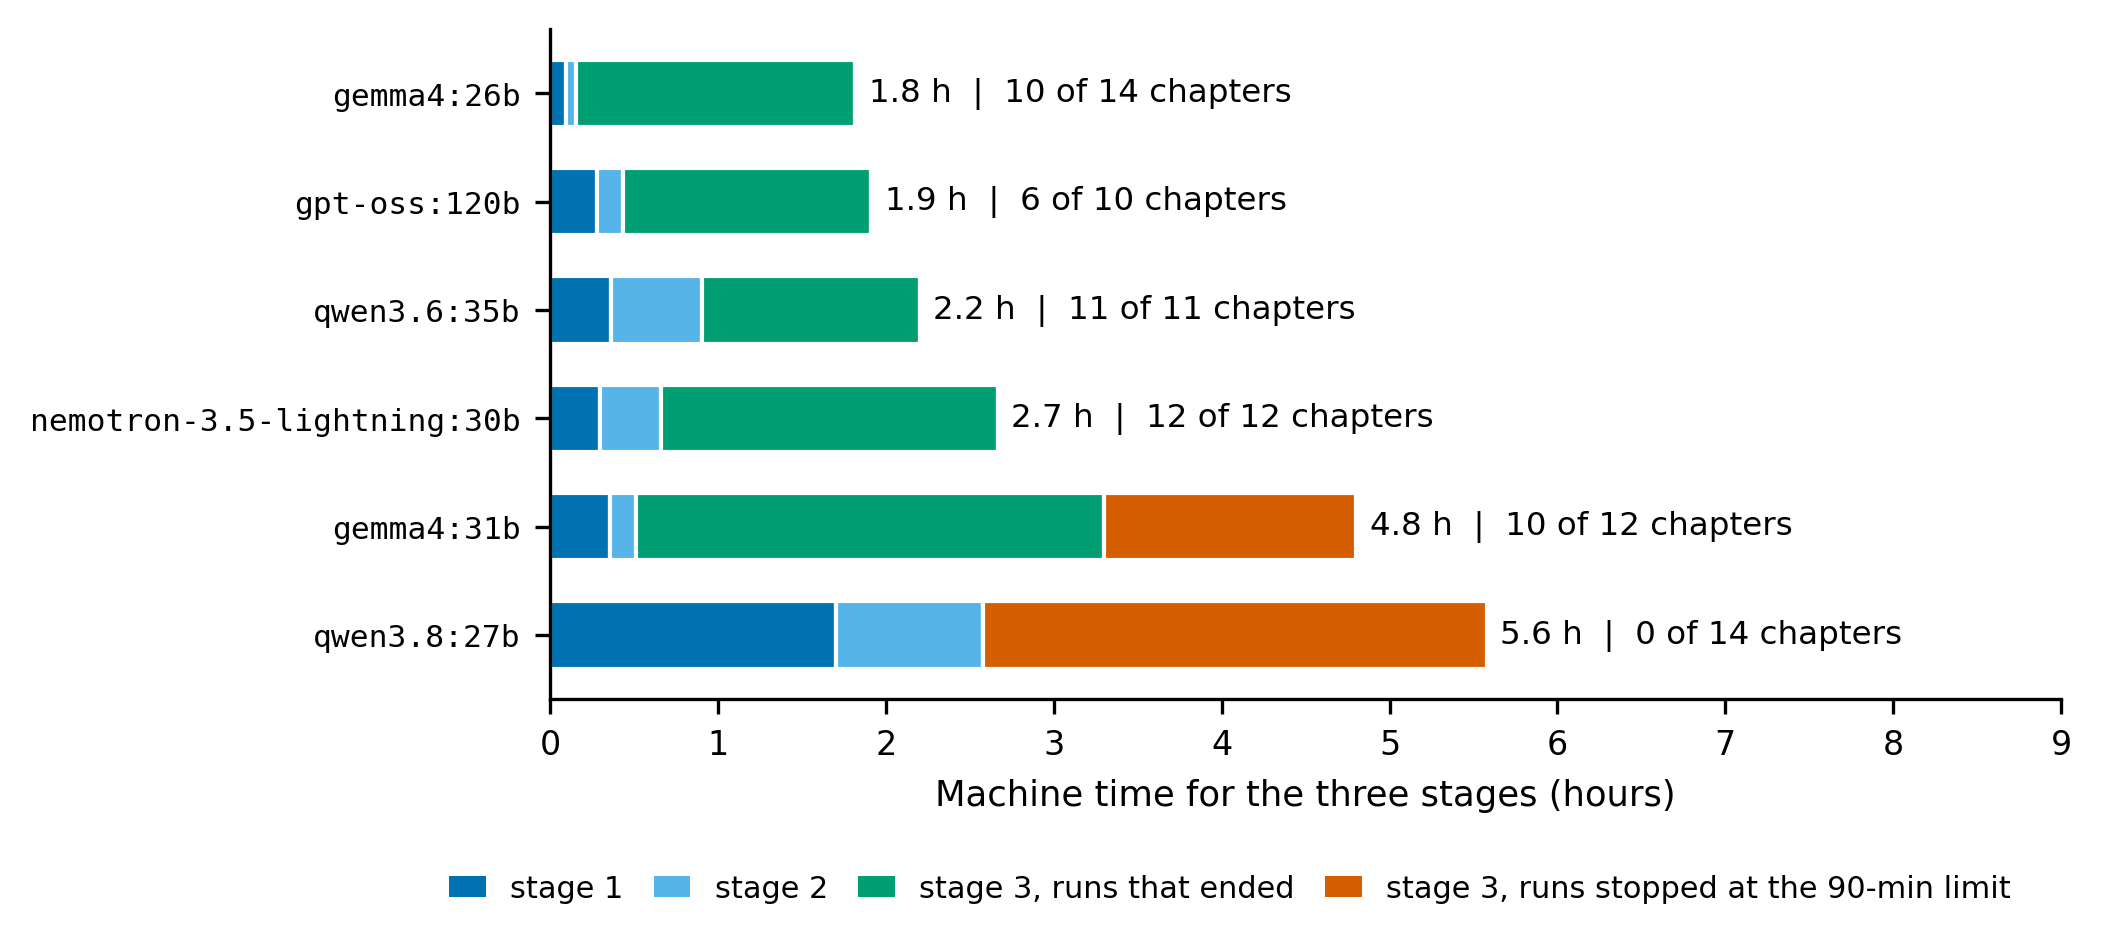
\includegraphics[width=0.95\textwidth]{figures/fig-time.png}
\caption{Machine time for the three stages, by stage, for the six models that produced a graph. Red segments are chapter runs stopped at the 90-minute limit.}
\label{fig:time}
\end{figure}

\begin{table}[htbp]
\centering
\small
{\setlength{\tabcolsep}{5pt}\begin{tabular}{@{}lrrrrr@{}}
\toprule
\textbf{Model} & \textbf{Hours} & \textbf{Calls} & \textbf{Failed} & \textbf{Tokens (K)} & \textbf{Median chapter (min)} \\
\midrule
\Gtwentysix & 1.8 & 416 & 38 (9\%) & 303 & 7.4 \\
\Gptoss & 1.9 & 158 & 7 (4\%) & 108 & 10.1 \\
\Qsix & 2.2 & 465 & 33 (7\%) & 437 & 6.4 \\
\Nemo & 2.7 & 691 & 77 (11\%) & 532 & 8.3 \\
\Gthirtyone & 4.8 & 265 & 52 (20\%) & 171$^{*}$ & 14.1 \\
\Qeight & 5.6 & 128 & 2 (2\%) & 81$^{*}$ & 90 (limit) \\
\bottomrule
\end{tabular}}
\caption{Effort across the three stages. Output tokens are as reported by the server and include reasoning. $^{*}$A run stopped at the limit writes no result record, so its tokens are missing; for \Qeight{} the figure covers stages~1 and~2 only.}
\label{tab:effort}
\end{table}

Three details matter for planning. Tool-call failure rates ranged from 2\% to 20\%, and the model that had passed every format rule in isolation, \Gthirtyone, had the highest rate in the harness. Two models drove the conversation to the configured window: the server logged tasks of 163,832 tokens for \Nemo{} and 163,082 for \Qsix{} against a window of 163,840, so at least one task of each was at or near the limit. And on the server used, one model's per-turn cost was dominated not by generating but by re-reading: for \Qeight, the server restored a checkpoint just past the system prompt and re-read the rest of the conversation on each turn, adding one to two minutes per turn, and one turn spent 19 minutes, nearly all on reasoning. The cause was not identified.

\subsection{Chapter Conformance}
\label{sec:quality}

Table~\ref{tab:quality} gives the conformance scores of the five books with written chapters, and Figure~\ref{fig:quality} shows each chapter.

\begin{table}[htbp]
\centering
\small
{\setlength{\tabcolsep}{4pt}\begin{tabular}{@{}lrrrrrrr@{}}
\toprule
\textbf{Model} & \textbf{Written} & \textbf{Level} & \textbf{Consist.} & \textbf{Floor} & \textbf{Headline} & \textbf{Prose wds} & \textbf{Grade} \\
\midrule
\Qsix & 11 of 11 & 76.4 & 84.1 & 55.9 & \textbf{64.3} & 51,900 & 10.5 \\
\Gthirtyone & 10 of 12 & 69.8 & 91.1 & 68.7 & \textbf{63.6} & 16,137 & 9.4 \\
\Nemo & 12 of 12 & 66.1 & 79.3 & 35.2 & \textbf{52.5} & 52,792 & 11.5 \\
\Gtwentysix & 10 of 14 & 53.4 & 79.1 & 54.5 & \textbf{42.3} & 22,569 & 10.4 \\
\Gptoss & 6 of 10 & 40.9 & 95.3 & 63.5 & \textbf{39.0} & 5,658 & 9.6 \\
\Qeight & 0 of 14 & 0.0 & --- & --- & --- & --- & --- \\
\bottomrule
\end{tabular}}
\caption{Conformance of each book, scored on 49 written chapters. Level is the mean chapter score with stubs as 0; consistency is $100(1-\mathrm{CV})$ over written chapters; floor is the lowest written chapter; headline is level times consistency over 100. Prose words exclude specifications, code, and the concept table. Grade is the mean Flesch--Kincaid grade of the prose against a target of 9.0.}
\label{tab:quality}
\end{table}

\begin{figure}[htbp]
\centering
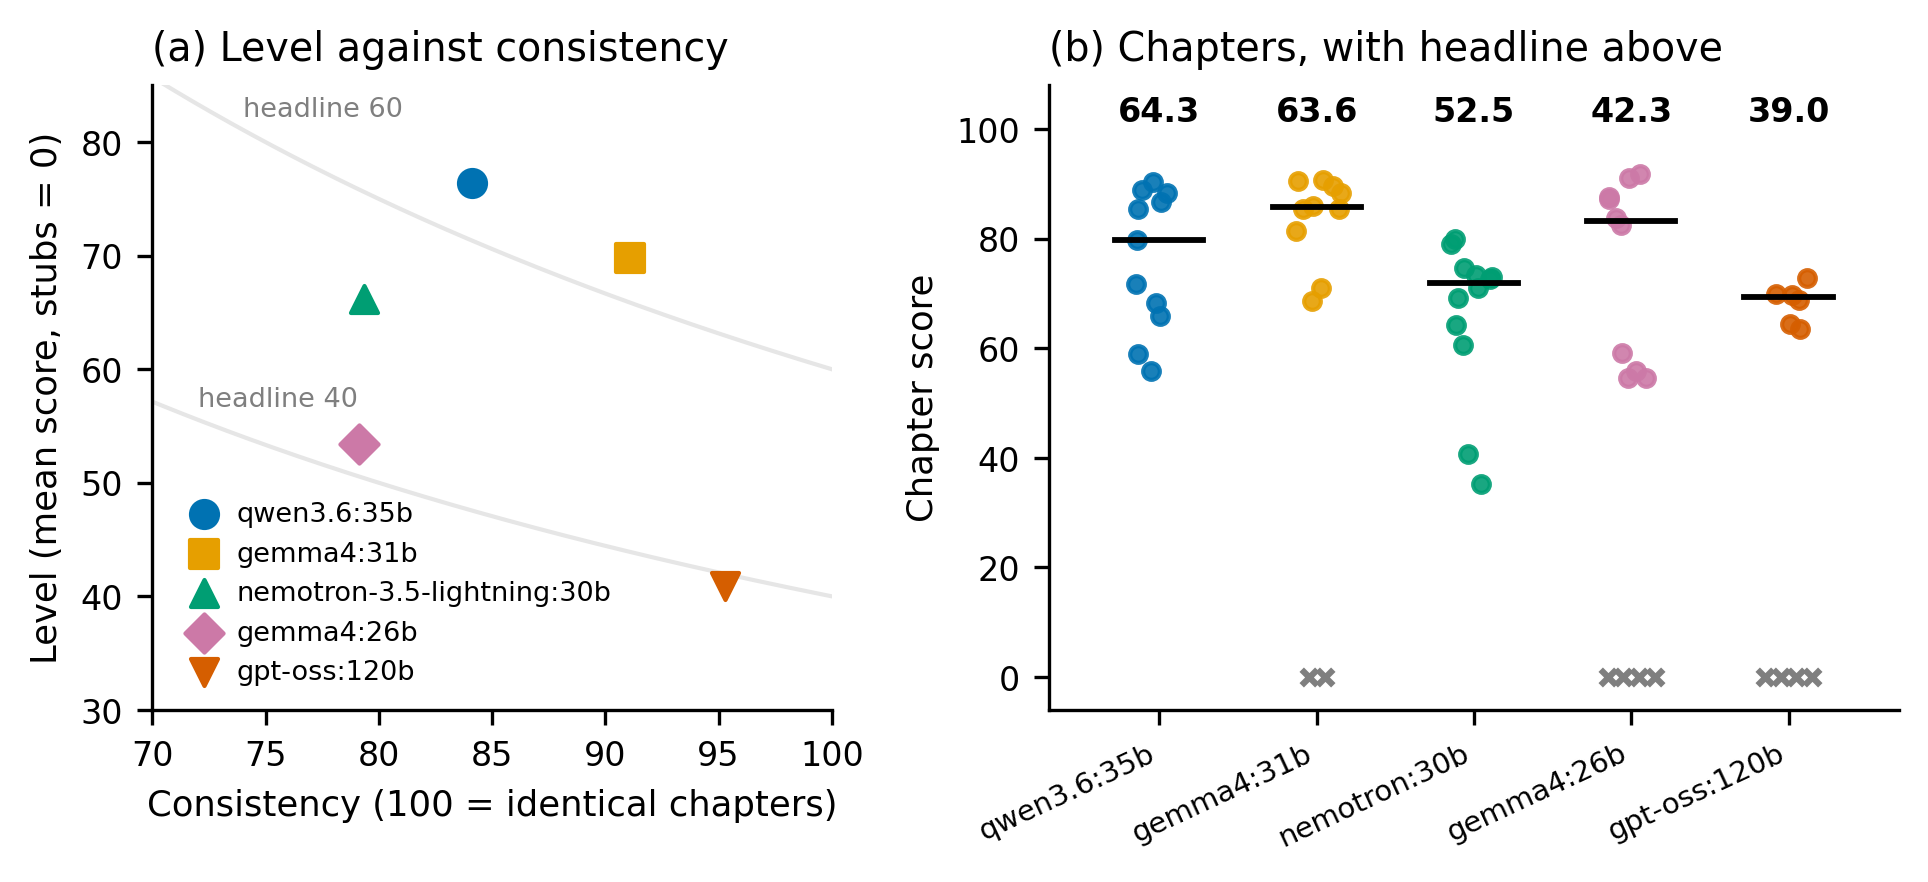
\includegraphics[width=\textwidth]{figures/fig-quality.png}
\caption{(a) Level against consistency; light curves are lines of constant headline. (b) Every chapter score; the bar is each book's median, a gray cross is an unwritten chapter scored 0, and the number above is the headline.}
\label{fig:quality}
\end{figure}

\paragraph{Ordering.}
\Qsix{} and \Gthirtyone{} are within a point of each other on the headline. Reweighting confirms they should be read as a tie: with each dimension weight perturbed by a uniform factor in $[0.6,1.4]$, the full ordering of the five books was unchanged in 61\% of 500 trials, and only two pairs ever swapped: \Qsix{} and \Gthirtyone{} in 39\% of trials, and \Gtwentysix{} and \Gptoss{} in 6\%. Beyond those pairs the order is stable: \Nemo{} stays third.

\paragraph{Level versus consistency.}
The headline separates two things that a mean would blur. \Gptoss{} has the highest consistency of any book, 95.3, because it wrote only six chapters and those six resemble each other; its level is the lowest. \Gthirtyone{} combines high consistency (91.1) with the highest floor (68.7) but lost two chapters. \Nemo{} has the lowest floor, 35.2, from two chapters that it wrote poorly, and the lowest consistency among books that wrote every chapter. This is the behavior the product was chosen to produce.

\paragraph{What the dimensions show.}
Table~\ref{tab:dims} gives the dimension means. Padding is near ceiling for every book (91 to 100), which is why its weight was lowered from 15 to 10: it adds points without separating anyone. Diagram placement and specification separate the books most, from 42 and 56 for \Nemo{} to 86 and 89 for \Gthirtyone. Reader fit is above 70 everywhere, but the mean reading grade of every book exceeds the target of 9.0, by 0.4 to 2.5 grade levels.

\begin{table}[htbp]
\centering
\small
\begin{tabular}{@{}lrrrrrr@{}}
\toprule
\textbf{Model} & \textbf{Budget} & \textbf{Placement} & \textbf{Spec.} & \textbf{Format} & \textbf{Padding} & \textbf{Reader} \\
\midrule
\Qsix & 66 & 64 & 79 & 78 & 100 & 88 \\
\Gthirtyone & 69 & 86 & 89 & 71 & 99 & 96 \\
\Nemo & 76 & 42 & 56 & 70 & 98 & 73 \\
\Gtwentysix & 83 & 51 & 57 & 88 & 96 & 93 \\
\Gptoss & 55 & 62 & 64 & 80 & 91 & 73 \\
\bottomrule
\end{tabular}
\caption{Mean dimension scores (0--100) over each book's written chapters.}
\label{tab:dims}
\end{table}

\paragraph{Book size.}
The two models that wrote every chapter wrote long books: \Nemo{} 81,700 words and \Qsix{} 75,400, about 6,800 words per chapter, against a reference of 55,000 words over 13 chapters (about 4,200 per chapter). The other three wrote about 2,600 to 3,000 words per chapter. Word counts must be read with care: most of \Gptoss's text is not prose. Of 17,890 words in its six written chapters, only 5,658 are prose; the rest is 108 diagram specifications, code, and concept tables. Thirty-one of those specifications are templated copies of a sibling, and in one chapter the misconceptions field of all twenty specifications reads, literally, ``(common misconceptions).'' A word-count threshold alone cannot see that.

\paragraph{Defects that a program found.}
Table~\ref{tab:defects} counts defects across written chapters. Each was confirmed by reading the chapter. The model's own working left in the text (a tier label such as \texttt{(Tier C: 120-200 words)}) occurs 127 times in \Nemo's chapters. Chapter titles that do not match their concept lists appear in five chapters each of \Nemo{} and \Gptoss. One embedded simulation points at an invented host. Lists with no blank line before them, which the site renders as a run-on paragraph, are the most common defect overall and are most frequent in \Gthirtyone{} (227), the book with the best placement and specification scores. Of 8,880 equations across all books, one is malformed: in a \Gthirtyone{} chapter that opens an equation with one delimiter and closes it with another, so the renderer swallows a sentence.

\begin{table}[htbp]
\centering
\small
\begin{tabular}{@{}lrrrrrr@{}}
\toprule
\textbf{Model} & \textbf{Lists} & \textbf{Leaks} & \textbf{Templated} & \textbf{Title} & \textbf{No diagram} & \textbf{Eq. ok/bad} \\
\midrule
\Qsix & 110 & 9 & 0 & 0 & 2 & 3,079/0 \\
\Gthirtyone & 227 & 0 & 0 & 0 & 0 & 1,065/1 \\
\Nemo & 141 & 127 & 0 & 5 & 2 & 3,294/0 \\
\Gtwentysix & 59 & 0 & 2 & 1 & 3 & 1,154/0 \\
\Gptoss & 19 & 20 & 31 & 5 & 0 & 288/0 \\
\bottomrule
\end{tabular}
\caption{Defects across written chapters. Lists: lists with no blank line before them. Leaks: pieces of the model's own working left in the text. Templated: specifications that copy a sibling. Title and No diagram: number of chapters with a title that matches none of its concepts, and with no diagram specification. Eq.: well-formed and malformed equations.}
\label{tab:defects}
\end{table}

\subsection{Summary of What the Results Support}

Four statements are supported by these runs. Six of ten open-weight models completed a learning graph on one 128~GB machine, in 6 to 102 minutes and, for five of them, within 22. Two completed every chapter they designed, in about 2.2 and 2.7 hours for all three stages. The failures that stopped the others were mostly of protocol and persistence. And a program can separate books whose chapters follow the rules evenly from books whose chapters do not, although the top two books should be read as a tie. Three statements are \textit{not} supported: that any chapter is correct, that any model would complete again on a second run, and that a local model matches a cloud model.
